\section{Misura delle caratteristiche di IC SN74LS244 }
\subsection{Caratteristiche statiche}
	Per tutta la sezione si è proceduto ad alimentare il circuito con una tensione
	\SI{5.01 \pm 0.01}{\volt}.
	\paragraph{Misvre delle tensioni d'operazione}
	Per effettuare la misura delle tensioni operative si
	è montato il circito in \figurename{ \ref{f:c1}}
		\begin{figure}[h]
			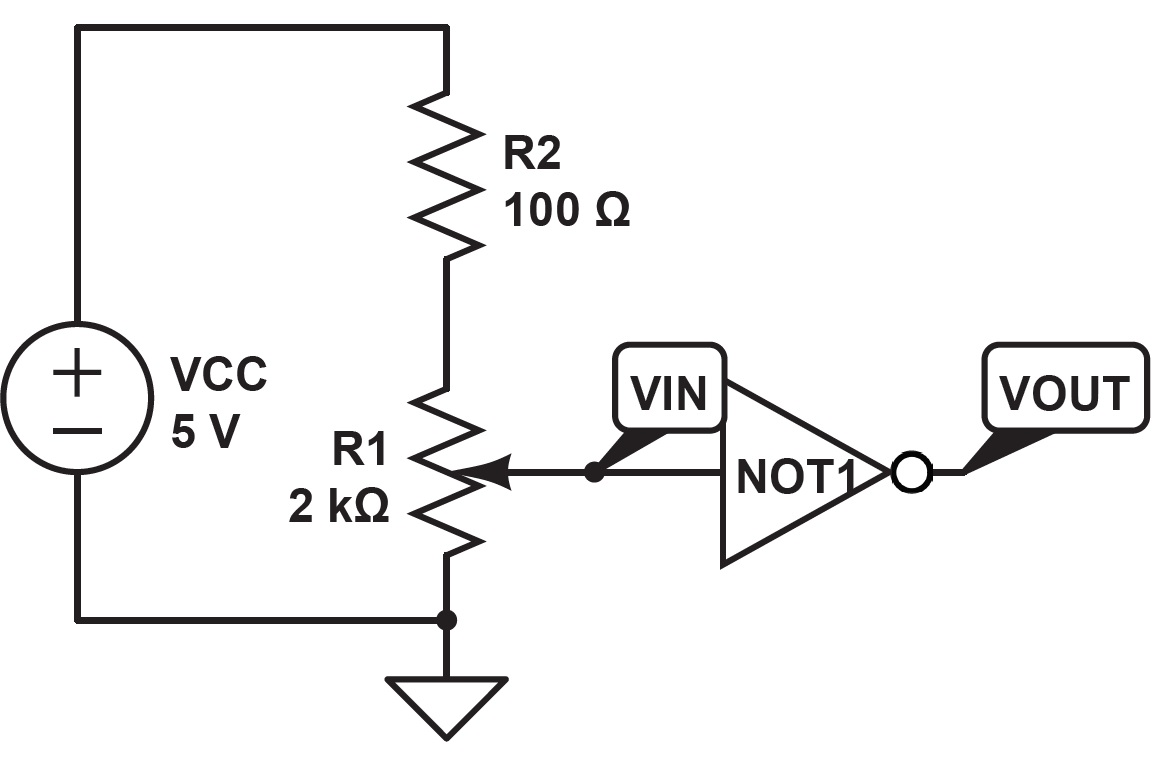
\includegraphics[scale=1.0]{immagine1.png}
			\caption{Rappresentazione del primo circuito impiegato.}
			\label{f:c1}
		\end{figure} .
	Andando a campionare la tensione in scita $V_{ot}$ in fnzione della tensione di ingresso  $V_{in}$.

	Il circito in  \figurename{ \ref{f:c1}} rappresenta n partitore di tensione;
		difatti variando la resistenza del trimmer $R_{1}$ si varia la tensione $V_{in}$.Per la costrzione si è impiegato n trimmer $R_{1}$ di valore massimale $R_{1}^{max}=$\SI{2 \pm 858}{\kilo \ohm} ed na resistenza $R_{2}=$\SI{100.8 \pm 0.1 }{ \ohm}.

	Si riportano i dati campionati in \tablename{ \ref{t:1}}
		\begin{table}[hb]
		\centering
		\begin{tabular}{S S}
			\toprule
			$V_{in}$ [\si{\volt}] & 	$V_{ot}$ [\si{\volt}]\\
			\midrule
			0 \pm 0.1 & 4.38 \pm 0.01\\
			0.265 \pm 0.001 & 4.23 \pm 0.01\\
			0.584 \pm 0.001 & 4.02 \pm 0.01\\
			0.780 \pm 0.001 & 3.87 \pm 0.01\\
			0.881 \pm 0.001 & 3.78 \pm 0.01\\
			0.945 \pm 0.001 & 3.44 \pm 0.01\\
			1.00 \pm 0.01 & 2.95 \pm 0.01\\
			1.065 \pm 0.001 & 2.0 \pm 0.01\\
			1.10 \pm 0.01 & 0.1773 \pm 0.0001\\
			1.238 \pm 0.001 & 0.1728 \pm 0.0001\\
			1.563 \pm 0.001 & 0.1728 \pm 0.0001\\
			1.775 \pm 0.001 & 0.1728 \pm 0.0001\\
			1.991 \pm 0.001 & 0.1727 \pm 0.0001\\
			2.52 \pm 0.01 & 0.1727 \pm 0.0001\\
			3.02 \pm 0.01 & 0.1726 \pm 0.0001\\
			3.48 \pm 0.01 & 0.1726 \pm 0.0001\\
			3.93 \pm 0.01 & 0.1726 \pm 0.0001\\
			5.00 \pm 0.01 & 0.1726 \pm 0.0001\\
			\bottomrule
		\end{tabular}
		\caption{Si riportano i valori corrispondenti alle nostre acqisizioni.I dati campionati sono stati ottenti col mltimetro digitale.
		Si è associato alle misre l'incertezza di n  digit slla prima cifra che risltasse instabile o qalora fossero ttti stabili di n digit,a tali misre si devono aggingere eventali errori di calibrazione del mltimetro.}
		\label{t:1}
	\end{table}
	.
	Effettando n grafico  ( \figurename{ \ref{f:i1}} )
	 dei dati in  \tablename{ \ref{t:1}} sono stati osservati i valori:
	 $V_{I,H}$, tensione in ingresso associata all'scita HIGH;$V_{I,L}$, tensione in ingresso associata all'scita LOW;$V_{O,H}$,intervallo di tensione in scita   HIGH;$V_{O,L}$,intervallo di tensione in scita associata all'scita LOW.

	 Essendo tali valori da intendersi come intervalli di tensione si sono osservati i loro valori superiori ed inferiori.
	 Si ottiene :
	 \begin{center}
	 $V_{I,H}^{max}=$\SI{0.01 \pm 0.1}{\volt} \\
	 $V_{I,H}^{min}=$\SI{1.003 \pm 0.1}{\volt}\\
	 $V_{I,L}^{max}=$\SI{5.0 \pm 0.1}{\volt}\\
	 $V_{I,L}^{min}=$\SI{1.10 \pm 0.1}{\volt}\\

	 $V_{O,H}^{min}=$\SI{2.95 \pm 0.1}{\volt}\\
	 $V_{O,H}^{max}=$\SI{4.38 \pm 0.1}{\volt}\\
	 $V_{O,L}^{min}=$\SI{0.1726 \pm 0.1}{\volt}\\
	 $V_{O,L}^{max}=$\SI{0.1773 \pm 0.1}{\volt}	\\
	 \end{center}

	 Tali stime risltano essere meno restrittivi dei i valori
	 nominali forniti dal costrttore nel datasheet.Si impta qesta lieve discrepanza
	 col fatto che i valori forniti dal datasheet siano fornite nelle peggiori condizioni di operatività possibili:
	 \begin{center}

	 	$V_{O,H}^{min,atteso}=$\SI{2.4}{\volt}\\
	 	$V_{O,L}^{max,atteso}=$\SI{0.4}{\volt}\\
	 $V_{I,H}^{min,atteso}=$\SI{2}{\volt}\\
	 $V_{I,L}^{max,atteso}=$\SI{0.8}{\volt}\\
 \end{center}
	 Si osserva che nella regine di tensione compresa tra 	$V_{I,L}^{max}$ ed $V_{I,H}^{min}$ il segnale in uscita non rislta essere forzato ne nella regione $V_{O,H}$ o $V_{O,L}$, risltando pertanto  l'scita indeterminata tra il regime di scita high e low.
	\begin{figure}[h]
		\centering
		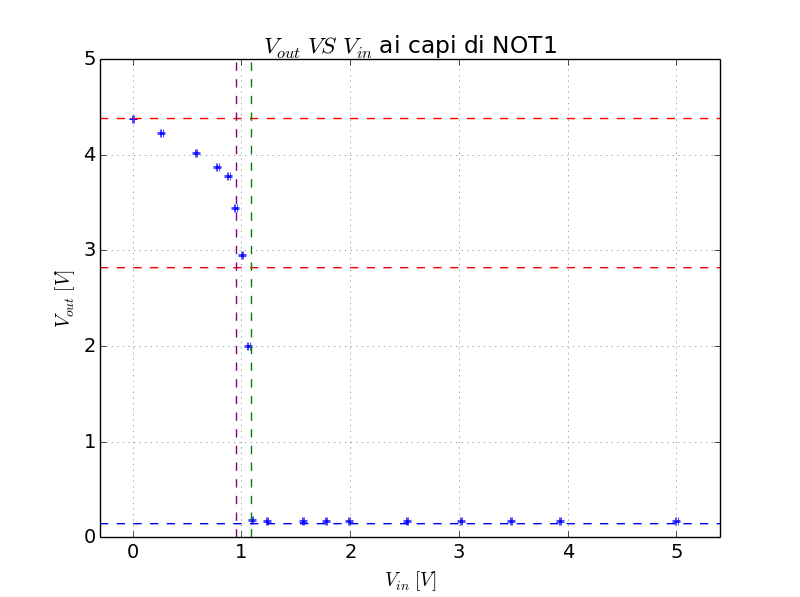
\includegraphics[scale=0.50]{in-ot.png}
		\caption{Rappresentazione dei dati in \tablename{ \ref{t:1}}.}
		\label{f:i1}
	\end{figure}


\paragraph{Misura delle correnti e stima del fanout}
	Si è proceduto dapprima alla misura delle correnti in ingresso.
	Per fare ciò si è modificato il circuito in \fig{i1} inserendo in serie tra il trimmer e la porta logica il multimetro in configurazione amperometro.

	Avendo assunto che il fabbisogno di corrente della porta logica dipenda 	dallo stato di funzionamento (ingresso alto o ingresso basso)
	si è andati a imporre un segnale di $V_{IH} = \SI{4.73\pm 0.03}{\volt}$ osservando una corrente $I_{IH} \lesssim \SI{0.5}{\micro \ampere}$ (si è scelto di usare il multimetro digitale come voltmetro per la misura di $V_I$ ed il multimetro analogico come amperometro per la misura di $I_I$, dal momento che quest'ultimo è in grado di misurare correnti molto più basse, ma $I_{IH}$ resta troppo piccola per poter essere misurata, con uno spostamento dallo zero inferiore alla mezza tacca con il fondoscala più basso disponibile);
	analogamente si è posto per la misura di  $I_{IL}$ una tensione in ingresso $V_{IL} =$ \SI{0.1525(1)}{\volt} rilevando una corrente di \SI{-25(1)}{\micro \ampere}. Si sono poste positive le correnti entranti nella porta logica e consegentemente negative quelle uscenti.

	Al variare della tensione in ingresso $V_{I}$ rimanendo entro il rispettivo range di funzionamento per ingresso alto o basso le correnti rilevate non cambiano significativamente; tali valori sono ampiamente entro i valori massimi riportati dal datasheet.
	Come ci aspettiamo per porte realizzate con	logica TTL, le correnti a linea bassa sono molto più alte di quelle a linea	alta.

	Si è proceduto dunque alla misura delle correnti in uscita $I_{OL}$ ed $I_{OH}$, ovvero rispettivamente quelle rilevate in uscita alla porta logica per lo stato di output basso ed output alto; per fare ciò si è montato il circuito in \fig{c2}.

	\begin{figure}[h]
		\centering
		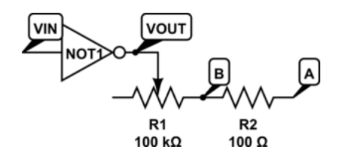
\includegraphics[scale=0.75]{cir2.png}
		\caption{Circuito impiegato per la misurazione di $I_{OL}$ e $I_{OH}$. }
		\label{f:c2}
	\end{figure}

	Dove i valori misurati dei componenti utilizzati sono:\\
	$R_{2} = \SI{100.8 \pm 1.1}{\ohm}$\\
	$R_{1,max} = \SI{94.0 \pm 0.9 }{ \kilo \ohm}$\\

	Per ottenere le correnti in uscita si è misurata la caduta di potenziale  $V_2$ ai capi di $R_{2}$ con il multimetro digitale; per effettuare le misure di $I_{OL}$ si sono posti $V_{in}$ e $V_A$ alla tensione di alimentazione $V_{CC}=$\SI{5.01 \pm 0.04}{\volt}, mentre per $I_{OH}$ si sono poste le tensioni precedenti a terra. La convenzione sui segni è la
	stessa della misura della corrente in ingresso: le correnti entranti
	nel dispositivo sono positive, quelle uscenti negative.

	Si osserva in entrambi i casi come al variare della resistenza del
	potenziometro la corrente vari dapprima lentamente per poi aumentare
	bruscamente (supponiamo al raggiungimento dei limiti del dispositivo) in
	corrispondenza del discostarsi della tensione in uscita dall'intervallo di
	corretto funzionamento; le misure raccolte sono riportate in \tab{iout}.

	\begin{table}[h]
		\centering
		\begin{tabular}{SS cc SS}
			\toprule
			\multicolumn{2}{c}{Uscita bassa} &&& \multicolumn{2}{c}{Uscita alta} \\
			\cmidrule(lr){1-2} \cmidrule(lr){5-6}
			{$I_{OL}$ [\si{\mA}]}	& {$V_{out}$ [\si{\V}]}	&&& {$I_{OH}$ [\si{\mA}]}	& {$V_{out}$ [\si{\V}]} \\
			\midrule
				0.0506 (25)	&	0.1758 (10)	&&&	-0.0437(24)	&	4.12 (3)	\\
				0.268 (5)	&	0.1868 (10)	&&&	-0.087 (3)	&	3.93 (3)	\\
				0.328 (5)	&	0.1904 (11)	&&&	-0.127 (3)	&	3.77 (3)	\\
				1.553 (18)	&	0.233 (2)	&&&	-0.164 (4)	&	3.63 (3)	\\
				2.90 (5)	&	0.266 (2)	&&&	-0.294 (5)	&	3.53 (3)	\\
				5.21 (7)	&	0.320 (3)	&&&	-3.77 (6)	&	3.28 (3)	\\
				24.0 (4)	&	1.891 (10)	&&&	-13.31 (15)	&	2.30 (2)	\\
				27.9 (5)	&	1.988 (11)	&&&	-16.91 (19)	&	1.860 (10)	\\
			\bottomrule
		\end{tabular}
		\caption{Andamento dell'uscita della porta not al variare della corrente erogata.}
	\label{t:iout}
	\end{table}

	La porta logica sembra dunque non poter essere utilizzata correttamente con
	uscita bassa per correnti $I_{OL}$ maggiori di $\sim \SI{5.5}{\mA}$, mentre
	ad uscita alta la situazione è meno chiara: sebbene l'uscita sia
	ragionevolmente stabile al variare del carico solo al di sotto di
	$\sim \SI{0.3}{\mA}$, $V_{out}$ resta entro valori tipici fino a correnti
	di qualche \si{\mA}, ed è sufficientemente alta da essere riconosciuta
	come tale in ingresso a porte logiche con simili caratteristiche (il
	datasheet dell'integrato da noi analizzato richiede una tensione alta in
	input di almeno \SI{2}{\V}, ma come mostrato nella sezione precedente il
	dispositivo è in realtà ben più generoso) fino ad oltre la decina di \si{\mA}.
	Ci attendiamo comunque che in tali condizioni la porta logica possa essere
	instabile, ed è certamente grandemente sensibile a piccole variazioni del
	carico, dunque un limite di corretto funzionamento si dovrà attestare
	su valori di $I_{OH}$ non maggiori di pochi \si{\mA}.

	Tali stime risultano maggiori dei valori limite riportati dal datasheet;
	ciò è probabilmente dovuto alla necessità del produttore di avere un certo
	margine d'errore, ma è anche possibile che la discrepanza sia imputabile
	alla minor severità delle condizioni di test: nel valutare le correnti in
	uscita si sono infatti mantenute sia $V_{cc}$ che $V_{in}$ lontane dai
	valori limite ammessi dall'integrato, ed è plausibile che avvicinandovisi
	il dispositivo sia meno tollerante nelle correnti erogabili.

	Con una corrente in ingresso che non supera (in modulo) i \SI{25}{\uA} ed
	una corrente erogabile certamente non inferiore a \SI{0.3}{\mA},
	una singola porta può fornire il proprio output in ingresso ad una dozzina
	di porte simili senza manifestare problemi. Questo è tuttavia un lower bound
	erroneamente basso: se teniamo conto del fatto che \SI{25}{\uA} assorbiti
	corrispondono ad un ingresso basso e ad uscita bassa la porta è certamente
	in grado di	erogare fino a $\sim \SI{5.5}{\mA}$, il fanout è di centinaia
	di porte in questa configurazione; anaolgamente, confrontando la corrente
	emessa ad ingresso alto ($\lesssim \SI{0.5}{\micro \ampere}$) con la
	corrente sopportabile ad uscita alta ($ > \SI{0.3}{\mA}$) otteniamo un
	fanout non inferiore alle 600 porte (ma probabilmente sensibilmente
	maggiore): prendendo il minore dei due come fanout effettivo della porta,
	dovrebbe dunque essere possibile utilizzare una singola porta per
	controllarne altre 220.


\section{Montaggio ardvino}
	Per la verifica delle caratteristiche dinamiche dell'IC SN74LS244 si è montato n circito implsatore con il microcontrollore arduino.
	Si riporta lo schema circitale in \figurename{ \ref{f:impulsatore}}.

		\begin{figure}[htb]
			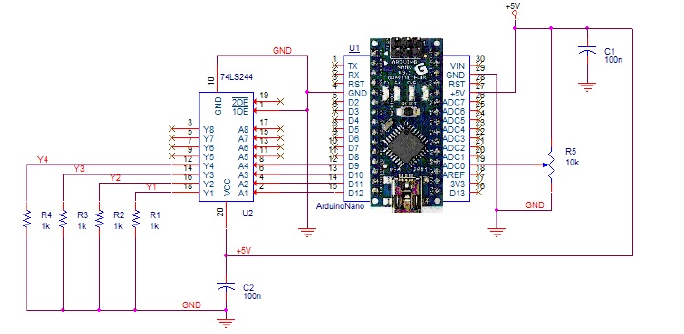
\includegraphics[scale=0.50]{imp.png}
			\caption{Rappresentazione del circuito impulsatore montato.}
			\label{f:impulsatore}
		\end{figure}
	Per il montaggio si sono impiegati le  segenti componenti circitali,riportate con la stessa notazione dello schema:
	\begin{center}
	\bigskip
		$R_{1}=$\SI{7.2 \pm 0.1}{\ohm} $R_{2}=$\SI{7.2 \pm 0.1}{\ohm} $R_{3}=$\SI{7.2 \pm 0.1}{\ohm} \\
		$R_{4}=$\SI{7.2 \pm 0.1}{\ohm} n trimmer di $R_{5}^{max}=$\SI{7.2 \pm 0.1}{\ohm} \\
 		dei condensatori	$C_{1}=$\SI{7.2 \pm 0.1}{\coulomb} $C_{2}=$\SI{7.2 \pm 0.1}{\coulomb}

	\end{center}
	Tale circito tra i terminali Y1 e Y2 dovrebbe generare dellle onde qadre sfasate di $\pi/2$ e freqenza compresa tra 50 Hz e 50KHz regolabile attraverso il valore di $R_{5}$.
	Si è andati pertanto a verificarne il corretto montaggio attraverso la verifica di qeste proprietà.
	Attraverso l'oscilloscopio si sono visalizzati s ch1 la tensione rilevata s Y1 e s  ch la tensione letta s Y2; si riporta na tipica acqisizione in
	\figurename{ \ref{f:oscil} } .
	\begin{figure}[htb]
		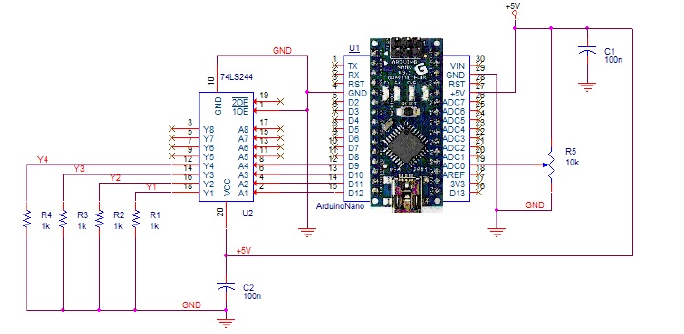
\includegraphics[scale=0.50]{imp.png}
		\caption{Tipica acqisizione delle tensioni lette si terminali Y1 (ch1) e Y2 (ch2) del circito implsatore.}
		\label{f:oscil}
	\end{figure}
	Come è possibile osservare dall'acqisizione la forma d'onda presentata dalle de tracce po essere trattata qale n onda qadra; si è inoltre osservato che al variare della resistenza la freqenza delle tracce assmeva valori compresi nell'intervallo $f\in [\sim 1 \text{Hz;} \sim 50 \text{KHz}]$.
	Come ltima verifica dell'operatività del circito montato si e procedto a misrare lo sfasamento tra le de traccie;
	per fare ciò si è andati a misrare $\Delta t$ tra i fronti di salita delle de
	 traccie, ottenendo $\Delta \cdot t=$\SI{41 \pm 55}{\sec} a fronte di na freqenza
	  $f=$\SI{59534 \pm 45}{\hertz}.
	Essendo valida la relazione \begin{equation}
	\Delta \phi = 2 \pi f \Delta t
	\end{equation}\label{eq:sfas}
	si ottiene $\Delta \phi=$\SI{0.5 \pm 0.01}{\radian}.
	Si è assnta pertanto come verificato il corretto fnzionamento del circito implsatore montato.

\section{Caratteristiche dinamiche}
	SI vogliono studiare le caratteristiche dinamiche della porta NOT, per farlo si è inviata all'ingresso della stessa un' onda quadra (generata dalla scheda Arduino, configurata come al punto precedente) di frequenza  $f\sim$\SI{1}{\kilo \hertz} e tensione picco picco $V=$\SI{3.40 \pm 0.20}{\volt}.

	\subsection{Tempi di propagazione}
	Si è misurato il tempo $\Delta t_{PHL}$ che intercorre tra il centro del fronte di discesa all'ingresso e il centro del fronte di salita sull'uscita. Si è poi ripetuta la misura per $\Delta t_{PLH}$: il passaggio dal fronte di discesa (input) al fronte di salita (output).
	Per determinare il centro dei fronti di salita/discesa si è preso il punto in cui i segnali assumevano la metà del loro valore HIGH, ignorando quindi la presenza di overshoot e undershoot, visibili in \figurename{ \ref{f:ripple}}.

	\begin{figure}[H]
		\centering
		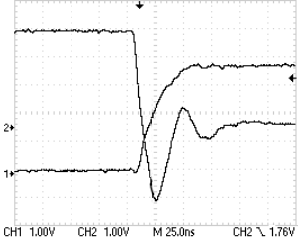
\includegraphics[scale=1]{undershoot_lh.png}
		\caption{Undershoot del segnale in uscita}
		\label{f:ripple}
	\end{figure}
	\noindent Per la misura si è scelta la scala che ottimizzava la risoluzione, ottenendo:
	$$\Delta t_{PHL}=\SI{9.6(6)}{\nano \second} \qquad \text{e} \qquad \Delta t_{PLH}=\SI{14.8(6)}{\nano \second}$$
	tali valori risultano in accordo con i valori attesi dal datasheet, che sostiene che entrambi i parametri debbano essere minori di \SI{15}{\nano \second}.

\subsection{Tempi di salita e discesa}
Si sono misurati i tempi di salita $\Delta t^{\uparrow}$ e discesa $\Delta t^{\downarrow}$ del segnale tra il $10 \% $ e il $90 \% $ del valore HIGH, sia in ingresso che in uscita. Si è ottenuto:
$$ \Delta t_{in}^{\uparrow}=\SI{12.2(6)}{\nano \second} \qquad \Delta t_{in}^{\downarrow}=\SI{6.4(6)}{\nano \second} $$
$$ \Delta t_{out}^{\uparrow}=\SI{16.4(6)}{\nano \second} \qquad \Delta t_{out}^{\downarrow}=\SI{48.8(1)}{\nano \second}.$$
